%% EAAI submission draft v3 -- elsarticle (author-year / elsarticle-harv).
%% v2 (2026-08-18) restructured after the organization of arXiv:2505.21574;
%% v3 (2026-08-18) reorganizes the body into Methodology (Sec. 3),
%% Experimental design (Sec. 4), and Results (Sec. 5). Claims and numbers
%% are unchanged (v1/v2 in main_v1_backup.tex / main_v2_backup.tex).
%% Compile: pdflatex -> bibtex -> pdflatex x2 (or upload to Overleaf).

\documentclass[preprint,12pt,authoryear]{elsarticle}

\usepackage{graphicx}
\usepackage{booktabs}
\usepackage{amsmath}
\usepackage{amssymb}
\usepackage{url}

\newcommand{\mapm}{mAP\(_{50\text{--}95}\)}

\journal{Engineering Applications of Artificial Intelligence}

\begin{document}

\begin{frontmatter}

\title{Allocation-aware inpainting augmentation for object detection:
class-set selection shapes where performance gains occur under a fixed
synthetic budget}

\author[a]{Daehyun Yoo}
\ead{dhyoo970111@gmail.com}
\affiliation[a]{organization={Affiliation to be completed},
                city={},
                country={Republic of Korea}}

\begin{abstract}
Synthetic images produced by diffusion inpainting can enlarge
object-detection training sets, but a practical question remains open:
given a fixed budget of generated images, which classes should receive
them? The artificial-intelligence contribution is a controlled answer to
this question. An allocation-aware
background-augmentation framework protects every annotated object,
regenerates only image backgrounds, and spends a fixed budget according
to an allocation signal --- a frequency-defined tail set
versus a weak set defined by validation average precision --- crossed
with a within-set weighting rule (uniform versus set-specific
priority); the four resulting arms are evaluated with pre-specified,
hash-frozen contrasts, seed-blocked tests, and multiple-comparison
correction. The engineering application is military aircraft detection
in two regimes: a 43-class natural-view benchmark and a 20-class satellite-view benchmark, paired
with a compact one-stage detector and a large pretrained transformer.
Three results follow. First, in the complete four-arm compact-detector
cells the allocation signal shapes where gains occur (set-by-scope
interaction $+0.06$, corrected $p = 0.017$; $+0.05$ on the satellite
benchmark, without multiplicity-adjusted significance), while priority weighting shows no
supported advantage over uniform quotas. Second, no measured arm shows a supported gain under the stronger
detector, whose standard-augmentation baseline exceeds the best
augmented compact model. Third, a generation-free
repeat-factor-sampling comparator produces larger mean gains than
inpainting on the deeply imbalanced benchmark but is null on the
shallower one, where inpainting retains consistently positive gains.
These findings yield a provisional engineering heuristic: check
baseline headroom, probe with resampling, then generate for the
measured-weakest classes with a uniform split. Code and artifacts will be
released.
\end{abstract}

\begin{keyword}
Data augmentation \sep Diffusion inpainting \sep Object detection \sep
Class imbalance \sep Synthetic data allocation \sep Military aircraft
detection
\end{keyword}

\end{frontmatter}

\section{Introduction}\label{sec:intro}

Object detectors in specialized domains often face uneven data
availability across classes: collecting and annotating representative
images is costly, and the resulting training sets are class-imbalanced.
Military aircraft detection is a useful case study because aircraft
types vary in visual similarity, prevalence, viewpoint, and background.
Diffusion-based synthesis offers one way to expand such training sets,
and generated images have improved classifiers
\citep{azizi2023synthetic, he2023synthetic} and detectors
\citep{suri2024gen2det, feng2024instagen}. For detection, recent work has
primarily improved the generation mechanism through conditioning,
filtering, diversity, and foreground or background editing; background
inpainting can preserve annotated foreground regions while varying their
surroundings \citep{li2024background}. Feedback-guided synthesis and
diffusion curricula have also begun to target underperforming or
underrepresented groups, mainly in classification settings
\citep{hemmat2024feedback, liang2025discl}. What has not been isolated in a controlled object-detection experiment
is whether class-set selection and within-set quota weighting
independently affect performance when the total budget, target-set
size, generator, and quality-control protocol are held fixed. We therefore ask two linked
questions:

\begin{quote}\itshape
Given a fixed budget of synthetic images, (i) which classes should
receive it --- the rarest classes or the classes with the lowest
validation performance --- and (ii) once that set is chosen, should the
budget be split uniformly or weighted by priority?
\end{quote}

The two class-selection policies need not agree. Frequency-based
allocation assumes that training frequency is an adequate proxy for the
classes that need additional support. In the exploratory analysis of
the natural-view Military Aircraft Detection (MAD) benchmark that
motivated our allocation hypothesis, however, the bottom-30\%
frequency set and the equally sized weak set --- selected by the
compact baseline's validation average precision (AP) averaged over
intersection-over-union (IoU) thresholds 0.50--0.95 --- turned out to
be disjoint. Some rare aircraft types are visually distinctive, whereas several of the
lowest-AP classes occur in the middle or head of the frequency
distribution. In this benchmark, ``help the rare'' and ``help the weak''
are therefore competing allocation policies rather than synonyms. This
separation is an empirical property of the studied data, not an assumed
law relating frequency and difficulty.

We study these choices with an allocation-aware background-augmentation
framework (Figure~\ref{fig:pipeline}). Following the background
inpainting mechanism of \citet{li2024background}, every annotated box is
protected during generation and its source pixels are restored
afterwards. This preserves the geometry and appearance of existing
annotations, although it cannot guarantee that no new, unlabeled object
appears in the regenerated background; we quantify that failure mode
with a detector-based audit and object-gate retraining. The allocation
framework distributes a fixed budget of $B$ images over a target set
chosen by an \emph{allocation signal} (frequency-defined tail vs.\
validation-AP-defined weak) and a \emph{within-set weighting} (uniform
vs.\ set-specific priority). Budget, set size, generator, prompts, and
rule-based verification are fixed, yielding four crossed allocation
arms. The priority score is set-specific, so weighting is compared
within each selected class set rather than interpreted as a single
global main effect. The AI contribution is therefore not a new
diffusion generator, but a controlled framework that separates which
classes receive synthetic data from how the quota is divided among them.
Because the allocation hypothesis originated in that exploratory MAD
phase, we time-stamped and hash-froze the five planned MAD contrasts
before training the four confirmatory augmentation arms or computing
any confirmatory-arm test-split metric. The resulting MAD experiment
therefore provides a prospectively specified, seed-level evaluation of
newly trained augmentation arms on the same benchmark, with inference
based on seed-blocked tests and Holm correction. We then
repeated the four-arm design on the separately prepared MAR20
(Military Aircraft Recognition) dataset,
whose allocation plan and contrasts were frozen before its untouched
official test split was evaluated, to assess cross-domain replication.

We evaluate the framework on two public military-aircraft benchmarks
with visually distinct imaging regimes: the 43-class natural-view MAD
and the 20-class satellite-view MAR20. Both use a compact one-stage
detector (YOLOv8n) for the complete four-arm design; reduced cells with a
larger pretrained transformer (RT-DETR-L) evaluate repeat-factor
sampling (RFS) and the two tail-set inpainting arms. Every included arm
is trained over three training seeds. Three findings emerge. First, on MAD the relative advantage of
the two arm families changes with evaluation scope (set-by-scope
interaction $+0.060$, Holm-adjusted $p = 0.017$), although the pooled
tail- and weak-arm improvements over baseline do not individually survive
Holm correction. MAR20 reproduces the direction and approximate
magnitude of the interaction ($+0.052$) but does not reach
multiplicity-adjusted significance (Holm-adjusted $p = 0.091$). Across the four within-set comparisons, priority weighting
shows no detectable benefit over a uniform split at the tested budgets;
the confidence intervals do not establish strict equivalence. Second,
in the reduced RT-DETR-L cells, all measured augmentation changes are
small and none is statistically supported against the
standard-augmentation baseline.
This association is consistent with reduced model headroom, but the
comparison also changes architecture and capacity and does not isolate a
causal mechanism. Third, generation-free RFS produces substantially
larger mean gains than the inpainting arms on the more imbalanced MAD
benchmark but provides no overall gain on the less imbalanced MAR20
benchmark. Because the datasets differ
in more than imbalance, this contrast motivates a practical hypothesis,
not a general diagnostic law.

Taken together, the study contributes (i) a fixed-budget formulation
that separates class-set selection from within-set weighting, (ii) a
multi-dataset, multi-detector evaluation that identifies where the
observed effects do and do not transfer, and (iii) a configuration-driven
artifact package containing allocation plans, generation logs,
per-class metrics, contrast freezes, and weights for 66 archived training
runs. The results suggest a provisional engineering heuristic: establish
a strong standard-augmentation baseline, test generation-free resampling,
and, when additional synthetic data are still warranted, target the
lowest-validation-AP classes with the simpler uniform allocation. Broader
datasets, capacity-matched detectors, and budget-scaling experiments are
needed before this heuristic can be treated as a general rule.

\section{Related work}\label{sec:related}

\subsection{Generative augmentation for detection and instance segmentation}
Building on denoising diffusion models \citep{ho2020ddpm,
rombach2022ldm}, synthetic data has supported image classification
through class-conditional generation \citep{azizi2023synthetic},
zero/few-shot recognition \citep{he2023synthetic}, and language-guided
editing \citep{trabucco2024dafusion, dunlap2023alia}. For detection and
instance segmentation, existing approaches differ chiefly in
\emph{where} synthetic content is introduced and \emph{how} localization
labels are obtained. Instance-composition methods paste real or generated
object cutouts into new scenes: Copy-Paste established the basic recipe
\citep{ghiasi2021copy}; X-Paste scaled it with text-to-image generation
and zero-shot filtering \citep{zhao2023xpaste}; MosaicFusion and DiverGen
extended generated-object augmentation to long-tailed instance
segmentation, with the latter emphasizing category, prompt, and generator
diversity \citep{xie2025mosaicfusion, fan2024divergen}; and SOC recently
scaled object-centric composition while preserving annotation accuracy
across detection, segmentation, and grounding \citep{huang2026soc}.
Full-scene and region-controlled methods
instead synthesize images together with localization cues. InstaGen adds
an instance-level grounding head \citep{feng2024instagen}, Gen2Det couples
grounded scene generation with image- and instance-level filtering
\citep{suri2024gen2det}, ODGEN adapts a layout-conditioned generator to
domain-specific detection data \citep{zhu2024odgen}, AeroGen specializes
layout-conditioned generation for remote sensing
\citep{tang2025aerogen}, and ReCon improves region--text alignment during
sampling without retraining the generator \citep{zhu2025recon}. These
methods primarily optimize where and how content is synthesized, or how
labels remain aligned; they do not isolate how a fixed generation
budget should be distributed across classes.

Closest to our generation mechanism is background editing:
\citet{li2024background} protect annotated foregrounds and regenerate
their surroundings with Stable Diffusion inpainting, reporting improved
robustness and generalization across their detection benchmarks. We adopt
this mechanism to preserve existing object pixels and bounding-box
geometry; it does not guarantee annotation completeness because a new,
unlabeled object may appear in the regenerated background. We hold this
generation mechanism fixed and study the allocation policy on top of
it, rather than proposing another generator.

\subsection{Long-tailed detection: resampling and rebalancing}
The long-tail literature --- see \citet{oksuz2021imbalance} and
\citet{zhang2023longtail} for surveys --- conventionally uses class
frequency to characterize imbalance. LVIS introduced a large-vocabulary
benchmark, the rare/common/frequent reporting convention, and
repeat-factor sampling (RFS), a standard image-level resampling scheme
\citep{gupta2019lvis}; instance-aware and exponentially weighted
frequency refinements followed \citep{yaman2023irfs,ahmed2025eirfs}.
Methods developed across long-tailed recognition and detection also
rebalance losses or classifiers, including class-balanced reweighting
\citep{cui2019classbalanced}, equalization and group-softmax losses
\citep{tan2020equalization,li2020bags}, Seesaw loss
\citep{wang2021seesaw}, equalized focal loss for one-stage detectors
\citep{li2022efl}, and decoupled classifier retraining
\citep{kang2020decoupling}. Two implications shape our protocol. First,
evidence from a YOLOv5 study on a constructed long-tailed COCO subset
shows that mosaic and mixup can yield larger gains than sampling- and
loss-based corrections \citep{crasto2024imbalance}. We therefore measure
each evaluated RFS and inpainting intervention as a \emph{marginal}
addition to the same standard-augmentation baseline. Second, RFS-family
methods use frequency
as the signal for allocating training exposure, but frequency need not
coincide with empirical class difficulty. Accordingly, our protocol uses
RFS as a same-data, generation-free exposure comparator and treats
frequency
and empirical difficulty as distinct allocation signals.

\subsection{Allocating and selecting synthetic data}
Model feedback can enter a synthetic-data pipeline at several distinct
stages. In imbalanced classification, \citet{bozorgtabar2019informative}
use Bayesian active-learning scores to select informative cases for
class-aware GAN augmentation, whereas feedback-guided data synthesis uses
one-shot classifier feedback to steer diffusion sampling toward useful
examples \citep{hemmat2024feedback}. DisCL addresses a different decision:
it constructs a spectrum of image-guidance levels and schedules those
levels across training stages for long-tailed and low-quality
classification \citep{liang2025discl}. For long-tailed instance
segmentation, BSGAL instead uses a gradient cache to estimate the
downstream contribution of generated batches and select useful synthetic
examples \citep{zhu2024bsgal}. Most directly related, TADA selects
which \emph{examples} to augment by their training dynamics --- images
learned slowly early in training receive faithful diffusion
augmentation --- with gains reported mainly for classification and
preliminarily for object detection \citep{nguyen2026tada}; in
federated classification, budget-aware synthetic augmentation
distributes per-client generation budgets according to label skew
\citep{lee2026fedeas}.

Closest to class-wise allocation, MRCA jointly adapts per-class generation
counts, generated-object difficulty, and pasted-object size over multiple
rounds of long-tailed instance-segmentation training
\citep{kim2025mrca}. BSGAL therefore performs model-aware selection from
generated data, MRCA dynamically couples allocation and generation
across training rounds, and TADA selects individual examples by their
learning speed. Our protocol differs on both axes: the unit of
allocation is the \emph{class} --- selected by frequency or by
validation AP rather than by per-example training dynamics --- and the
design is deliberately static, pre-specifying and recording each
allocation plan before confirmatory training and comparing target-set
and within-set quota decisions at fixed $B$ and $K$ without adaptive
curation.

\subsection{Aircraft detection in natural and remote-sensing imagery}
Remote-sensing benchmarks span broad object detection, as in DOTA
\citep{xia2018dota} and DIOR \citep{li2020dior}, and fine-grained
oriented object detection, as in FAIR1M \citep{sun2022fair1m}. Military-aircraft
recognition has a dedicated large public benchmark in MAR20, which
contains 3{,}842 satellite images, 20 aircraft types, and both horizontal
and oriented box annotations \citep{yu2023mar20}. Architecture-centered
work includes the one-stage FGA-YOLO, evaluated on MAR20 and FAIR1M
\citep{wu2025fga}; related work in this journal addresses generic UAV
small-object detection through multi-scale attention
\citep{song2024small}. On the data side, class-specific diffusion
generation has recently been shown to improve military vehicle
detection in a low-data regime \citep{fokkinga2026military},
underlining the growing role of generative augmentation in this
domain.

Aircraft-specific work has also compared augmentation mechanisms.
\citet{shermaine2025compositing} evaluate classical augmentation, image
compositing, Stable Diffusion XL, and ControlNet with YOLOv8 on a custom
dataset of commercial and military aircraft. The public web-image MAD
dataset \citep{rookieengg2023mad} and satellite-view MAR20 benchmark
let us examine allocation in
two distinct imaging regimes, with selected policies additionally tested
across detector families.

\subsection{Positioning of this study}
Across these strands, prior work separately improves generation,
rebalancing, model-guided selection, and aircraft-specific augmentation.
To our knowledge, no prior object-detection study has factorially
compared equally sized frequency- and validation-AP-defined class sets
with alternative within-set quota rules under a common fixed-budget
pipeline. We address that
controlled policy comparison using four pre-specified arms: each target set is
paired with uniform quotas and its own pre-specified priority rule. Our
inference therefore concerns the two within-set
uniform-versus-priority contrasts of each full-design cell and the
set-by-scope interaction, not a universal weighting
main effect or a universally superior allocation signal.

\section{Methodology}\label{sec:method}

We first formalize the fixed-budget allocation problem
(Section~\ref{sec:prelim}). We then instantiate the allocation framework
with a deterministic quota allocator, a background-inpainting mechanism
that restores source-object regions before encoding and copies their
bounding boxes and class labels unchanged, and rule-based quality
verification
(Figure~\ref{fig:pipeline}; Sections~\ref{sec:alloc}--\ref{sec:verify}).
The pre-specified protocol for the primary confirmatory contrasts is
described as part of the experimental design in
Section~\ref{sec:stats}.

\begin{figure}[t]
\centering

\includegraphics[width=\linewidth]{figures/fig1_pipeline_design.pdf}
\caption{Framework overview. (a)~Generation pipeline: all annotated
boxes in a source image define padded protected regions; after
diffusion, source pixels are restored within those regions, and each
output must pass rule-based verification --- with budget refill
replacing rejected candidates --- before insertion into the training
split. Within each dataset's
four-arm full-design cell, budget $B$, class count $K$, generator,
prompt set, and verification rules are held fixed. (b)~The crossed
allocation design pairs each class set (frequency-defined tail or
validation-AP-defined weak) with uniform quotas and a set-specific
priority rule.}
\label{fig:pipeline}
\end{figure}

\subsection{Problem setup and notation}\label{sec:prelim}

\paragraph{Problem formulation}
Let $\mathcal{C}$ denote the class set of a detection dataset with
train/validation/test splits, and let $B$ and $K$ be fixed positive
integers denoting the synthetic-image budget and target-set size,
respectively. Here, $B$ counts the verified synthetic images added to
the training split, not failed generation attempts. A class-level
\emph{allocation plan} is a pair $(S,q)$, where
$S \subseteq \mathcal{C}$, $|S|=K$, and
$q=(q_c)_{c\in S}\in\mathbb{Z}_{>0}^{K}$ satisfies
$\sum_{c\in S}q_c=B$. Each accepted synthetic image is assigned to
exactly one target class $c$ for quota accounting and is generated from
a training image containing $c$; other annotated classes in the source
image are retained but do not count toward their quotas. We decompose
the plan into two decisions: the \emph{allocation signal} that selects
$S$ and the \emph{within-set quota rule} that determines $q$ given $S$.
A \emph{synthetic-augmentation arm} is the training condition obtained
by adding the $B$ accepted images specified by one plan to the training
split. The validation and test splits are never modified.

\paragraph{Evaluation scopes and metric}
Final performance is evaluated on the held-out test split using
per-class average precision averaged over intersection-over-union
thresholds 0.50--0.95. For arm $a$, seed $s$, and evaluation scope
$G \subseteq \mathcal{C}$, define
\[
M_{G,s}(a)=\frac{1}{|G|}\sum_{c\in G}\mathrm{AP}_{c,s}(a).
\]
We consider three scopes: \emph{all} ($G=\mathcal{C}$), the
frequency-defined \emph{tail} set, and the validation-AP-defined
\emph{weak} set. Weak-scope provenance, including reuse of the frozen
compact-detector scope in the MAD transformer cell, is specified in
Section~\ref{sec:alloc}. Let $a_0$ denote that cell's
standard-augmentation baseline (\texttt{basic\_aug}). For every
within-cell arm comparison, the reported gain is the paired seed-level
difference
\[
\Delta_{G,s}(a)=M_{G,s}(a)-M_{G,s}(a_0).
\]
Point estimates aggregate these seed-level values; the inferential
procedure is specified in Section~\ref{sec:stats}.

\paragraph{Resampling comparator}
Following \citet{gupta2019lvis}, we implement repeat-factor sampling
(RFS) as a generation-free, same-data comparator. Let $f(c)$ be the
fraction of training images containing class $c$. We define
\[
r(c)=\max\!\bigl(1,\sqrt{t/f(c)}\bigr),
\qquad
r(I)=\max_{c\in I}r(c).
\]
The threshold was fixed at $t=0.1$ after pilot pipeline calibration;
the initially considered value of $0.01$ produced no repetitions under
the observed training-set frequencies. For each image, the fractional
part of $r(I)$ is stochastically rounded with a fixed
dataset-construction base seed $s_0$, and the resulting repetitions are
materialized as image--label copies. This adds 8{,}930 copies on MAD (9{,}430 to 18{,}360 effective
training images) and 289 on MAR20 (1{,}064 to 1{,}353), whereas the
synthetic arms add 1{,}000 and 500 images, respectively. RFS is therefore
neither synthetic-budget- nor training-exposure-matched to the four-arm
design and is interpreted only as a separate exposure comparator. The
RFS arm otherwise retains the standard training-time augmentation used
by \texttt{basic\_aug}.
Because RFS introduces no new image content, it provides a same-data
diagnostic of whether re-exposure to existing labeled images is
sufficient to improve detection; it is not treated as a strict causal
decomposition of exposure and content variation
(Section~\ref{sec:r3}).

\subsection{Allocation signals and within-set quota rules}\label{sec:alloc}

In each full-design cell, we cross two target-set signals with two
within-set quota rules to obtain four augmentation arms:
\begin{itemize}
\item \textbf{Tail set (frequency signal).} Let
  $K=\lceil0.3|\mathcal{C}|\rceil$. The tail set contains the $K$
  classes with the fewest training instances. A pre-specified
  requirement of at least five validation instances ensures that
  per-class validation and scope metrics are estimable; this requirement
  did not alter the selected sets in either dataset.
\item \textbf{Weak set (difficulty signal).} Let
  $\overline{\mathrm{AP}}_c$ denote the per-class validation AP of the
  corresponding \texttt{basic\_aug} baseline, averaged over the
  0.50--0.95 intersection-over-union thresholds and over its three
  training seeds. The weak set contains the $K$ classes with the lowest
  $\overline{\mathrm{AP}}_c$. Thus, target-set size is held fixed while
  target-set identity changes. For the MAD full-design experiment,
  weak-set membership was frozen from the preceding exploratory
  validation results; the MAR20 full-design weak set was determined from
  its own baseline validation results before evaluation on the official
  test split. The reduced transformer cells do not train weak-targeted
  arms, so their weak sets serve only as descriptive reporting scopes.
  The MAD transformer cell reuses the frozen compact-detector weak set
  for cross-detector comparability, whereas the MAR20 transformer scope
  is derived from that detector's own baseline validation results.
\item \textbf{Uniform allocation.} The integer budget $B$ is distributed
  as evenly as possible across the $K$ selected classes.
\item \textbf{Priority allocation.} Let
  $\operatorname{mm}_{A}(x_c)$ denote min--max normalization over class
  set $A$. For the tail set $S_t$, we define
  \[
  R_c=1-\operatorname{mm}_{S_t}\!\bigl(\log(1+n_c)\bigr),\qquad
  W_c^{(t)}=1-\operatorname{mm}_{S_t}(\overline{\mathrm{AP}}_c),
  \]
  and use $P_c^{(t)}=0.6R_c+0.4W_c^{(t)}$. For the weak set $S_w$, we
  use $P_c^{(w)}=1-\operatorname{mm}_{\mathcal{C}}
  (\overline{\mathrm{AP}}_c)$.
\end{itemize}
Because the two priority scores are defined differently, the
uniform-versus-priority comparison is evaluated separately within each
target set. We treat these as two pre-specified within-set contrasts,
rather than as levels of a common weighting factor, and therefore do
not estimate a weighting main effect across sets.

Given nonnegative allocation weights and feasible bounds
$Kq_{\min}\leq B\leq Kq_{\max}$, quotas are computed by a deterministic
capped largest-remainder allocator. Each class first receives
$q_{\min}$ images; the remaining budget is distributed proportionally
to the selected weights subject to $q_{\max}$. Fractional leftovers are
assigned in descending remainder order, with ties resolved by the fixed
input order. Consequently, each of the four synthetic arms satisfies
\[
\sum_{c\in S}q_c=B,
\qquad
q_{\min}\leq q_c\leq q_{\max},
\]
holding the realized synthetic-image budget and target-set size
constant across the crossed comparison. Within the two full-design
cells, the frozen tail and weak sets overlap in 0 of 13 classes on MAD
and 1 of 6 classes on MAR20 (Section~\ref{sec:design}), confirming that
the two allocation signals select largely different target classes.

\subsection{Source-object-preserving background generation}\label{sec:generation}

Synthetic backgrounds are generated with the
\texttt{runwayml/stable-diffusion-inpainting} checkpoint
\citep{rombach2022ldm}, using FP16 inference on a GPU, 20 denoising
steps, guidance scale 7.5, and strength 0.85. Each source image and mask
is resized to a $512\times512$ working resolution, and the generated
image is resized back to the source dimensions. For every annotated
object, its bounding box is expanded by 10\% of the box width and height.
The inpainting mask marks pixels outside these padded boxes as editable
and uses a 12-pixel Gaussian-blurred transition band.

Because masking alone cannot guarantee unchanged object pixels, the
source pixels within every padded box are pasted back after diffusion
and before JPEG encoding. The original bounding-box coordinates and
class labels are copied unchanged. Object-region pixels are therefore
restored before encoding rather than claimed to be byte-identical in the
stored JPEG; post-encoding changes are checked by the verification
procedure in Section~\ref{sec:verify}. Dataset-specific prompt sets
contain five natural-view aviation prompts for MAD and five top-down
aerodrome prompts for MAR20. Their negative prompts discourage new
aircraft and other artifacts, but cannot guarantee annotation
completeness if a new object appears in the regenerated background.

Source selection and prompt assignment follow fixed cyclic schedules.
For target class index $c$, candidate index $i$, and within-candidate
retry $r$, the generation seed is
$s_{c,i,r}=s_0+100{,}000c+i+r$, where $s_0$ is the same
dataset-construction base seed used for the resampling comparator
(Section~\ref{sec:prelim}). This procedure supports reproducible
generation within a fixed model, software, and hardware environment;
archived generated files are reused directly across applicable
experiments. Examples appear in Figure~\ref{fig:examples}, with
additional source--generated pairs in Appendix~\ref{app:gen}.

\subsection{Rule-based quality verification and budget refill}\label{sec:verify}

Source images must first offer enough editable background for inpainting
to be meaningful (protected regions covering no more than 95\% of the
frame); sources failing this pre-check are excluded before generation.
Every generated image must then pass two quantitative checks: (i)~the
background changed substantially (mean absolute pixel difference $\geq
10$ gray levels outside the boxes), and (ii)~the protected interiors did
not change beyond a compression-noise tolerance ($\leq 5$ gray levels).
Each candidate is retried at most twice, after which the fixed cyclic
schedule advances to the next source--prompt pair; at most $2q_c$
candidates are evaluated for class $c$. If this bound is exhausted
before that class's quota is met, the run aborts before training rather
than admitting an underfilled arm. Consequently, every completed
synthetic arm has realized budget $B$. A run also aborts if more than
half of its logged candidate records fail, flagging generator
malfunction. As an additional audit --- reported as a robustness check,
not a filter --- a detector-based scan flags candidate
\emph{hallucinated} objects (off-mask detections) that diffusion
occasionally paints into backgrounds, and an
object-level gate variant retrains the arms with all affected images
removed (Section~\ref{sec:robust}).

\section{Experimental design}\label{sec:design}

The engineering application is military aircraft detection under two
operationally distinct imaging regimes: natural side/ground views and
overhead satellite imagery. In this setting, collecting balanced
class-specific imagery is costly, making the allocation of a limited
augmentation budget a practical engineering concern. Both benchmarks
are publicly available, facilitating independent evaluation and
replication.

\subsection{Datasets}
\textbf{MAD} \citep[Military Aircraft Detection, natural side/ground
views; public;][]{rookieengg2023mad} contains 11{,}788 images with
18{,}832 boxes over 43 aircraft types. The downloaded YOLO release
provides 9{,}430 training images and a 2{,}358-image validation
partition, but no separate test partition. We sort the source validation
images by file path and divide them equally into validation and held-out
test subsets, yielding a 9{,}430/1{,}179/1{,}179 train/val/test
split. The halving is deterministic but not stratified; empirically,
all 43 classes appear in every split.
\textbf{MAR20} \citep[Military Aircraft Recognition dataset, satellite
view; public;][]{yu2023mar20} contains 3{,}842 images with 22{,}341 boxes
over 20 aircraft types; we use its horizontal bounding-box annotations.
We preserve the official 2{,}511-image test split untouched for final
reporting and divide the official 1{,}331 training images into
1{,}064/267 train/val subsets, stratified by each image's primary
class (the most frequent class among its boxes) with a fixed split
seed.

We define the train-split imbalance ratio as the largest divided by the
smallest class instance count. By this measure, MAR20 is less imbalanced
than MAD (7.7 vs.\ 10.5), providing a second observational setting rather
than an isolated manipulation of imbalance: viewpoint, dataset scale,
and label taxonomy also change. Tail sets are derived from training
counts and shared across detectors within each dataset
(Section~\ref{sec:alloc}). Weak sets are baseline-dependent in the two
full-design compact-detector cells. In the reduced transformer cells,
the MAD weak reporting scope reuses the frozen compact-detector set for
cross-detector comparability, whereas the MAR20 scope is derived from
the transformer baseline. The tail and weak scopes are disjoint on MAD
(0 of 13 classes); on MAR20 they overlap in one of six classes for the
compact detector and two of six for the transformer.

\subsection{Detectors and training}
We use two detectors spanning an order of magnitude in capacity:
YOLOv8n, a compact one-stage detector of the You-Only-Look-Once (YOLO)
family (3.2M parameters), and RT-DETR-L, the large variant of the
Real-Time Detection Transformer \citep[32M parameters;][]{zhao2024rtdetr}.
Both are initialized from checkpoints pretrained on the Common Objects
in Context (COCO) benchmark \citep{lin2014coco}, so the cells differ in capacity and
architecture family, not in pretraining corpus. All runs share the same nominal
training configuration within the Ultralytics framework
\citep{jocher2023ultralytics}: $640\times640$ input, up to 50 epochs
with early stopping (patience 15), and framework-default remaining
hyperparameters; the batch size is fixed to 8 for RT-DETR-L and
resolved automatically for YOLOv8n. Test metrics are computed from the
validation-selected checkpoint (\texttt{best.pt}) of each run, under a
single evaluation harness for every run in every cell.
\texttt{real\_only} (framework augmentation disabled) is a
no-training-augmentation reference and \texttt{basic\_aug} (default
photometric/geometric augmentation) is the baseline all gains are
measured against. Every arm--cell combination is trained with three
training seeds; all statistics aggregate over seeds as described in
Section~\ref{sec:stats}.

In the MAD compact-detector cell, the \texttt{basic\_aug} and
\texttt{real\_only} runs were trained during the exploratory phase and
reused; the five augmentation arms of that cell were trained afresh in
the confirmatory phase. The nominal configuration was shared, but the
realized conditions of the two periods were not identical: the
automatically resolved YOLOv8n batch size depends on the training
hardware (143 in a reused baseline run versus 41 in a confirmatory arm
run), dataloader settings differ, and the Ultralytics versions embedded in
the archived checkpoints differ as well (8.4.87 and 8.4.92 across the
reused reference runs versus 8.4.115 for the confirmatory arms); the
remaining software environment (PyTorch, CUDA) was not preserved.
Baseline-relative deltas in that cell therefore compare runs from two
training periods (Section~\ref{sec:limitations}), whereas the
set-by-scope interaction compares only the contemporaneously trained
arms.

\subsection{Cells and budgets}
Table~\ref{tab:cells} summarizes the four dataset $\times$ detector
cells. The YOLOv8n cells run the complete four-arm crossed design plus RFS
and the two reference arms; the RT-DETR-L cells run a reduced design (baseline, RFS, and
the two tail-set arms) intended to test whether gains transfer to a
stronger detector rather than to re-estimate the interaction. The tail-uniform arm's pool depends only on the dataset and is shared
across the detector cells; the tail-priority arm's difficulty
component is recomputed
from each detector's own baseline validation AP, so its allocation is
detector-specific. The budgets are $B = 1{,}000$ ($K = 13$, $q_{\min} = 5$, $q_{\max} = 200$) for MAD and $B = 500$
($K = 6$, $q_{\min} = 5$, $q_{\max} = 100$) for MAR20,
which keeps the average per-class quota similar across datasets
($B/K \approx 77$ and ${\approx}\,83$). Because the training splits
differ in size, the synthetic-to-real ratio is not matched: the budget
amounts to 10.6\% of the MAD training split but 47.0\% of the much
smaller MAR20 split, so cross-dataset comparisons contrast allocation
policies at comparable per-class quotas, not at a matched
dataset-level dose. Realized budgets equal planned budgets in all
cells (verification failure rates per pool: 18.0--20.6\% of attempts
on MAD, 0.6--1.2\% on MAR20, absorbed by the refill mechanism of
Section~\ref{sec:verify}).

\begin{table}[t]
\centering
\caption{Experimental cells. All cells share the generation and
verification pipeline and the seed-blocked testing framework; each
cell carries a pre-specified contrast family (five contrasts in the
four-arm cells, three in the reduced cells; Section~\ref{sec:stats}).}
\label{tab:cells}
\small
\begin{tabular}{llp{0.42\linewidth}l}
\toprule
Dataset & Detector & Arms & Budget $B$\,/\,$K$ \\
\midrule
MAD   & YOLOv8n   & $2\times2$ arms + RFS + \texttt{basic\_aug} + \texttt{real\_only} & 1{,}000\,/\,13 \\
MAD   & RT-DETR-L & \texttt{basic\_aug} + RFS + tail-uniform + tail-priority & 1{,}000\,/\,13 \\
MAR20 & YOLOv8n   & $2\times2$ arms + RFS + \texttt{basic\_aug} + \texttt{real\_only} & 500\,/\,6 \\
MAR20 & RT-DETR-L & \texttt{basic\_aug} + RFS + tail-uniform + tail-priority & 500\,/\,6 \\
\bottomrule
\end{tabular}
\end{table}

\subsection{Pre-specified statistical protocol}\label{sec:stats}

We separate planning from evaluation: no allocation score or
class-set definition uses the test split --- training-set instance
counts define the tail set, and baseline validation AP defines the
weak set and the difficulty component of the priority scores --- and
the test split is reserved for final reporting. The MAD hypotheses and
contrast family themselves originated in the exploratory phase
disclosed in Section~\ref{sec:intro}. For the four-arm cells, five primary
contrasts were fixed --- with a content hash and timestamp --- before
any confirmatory-arm test-split metric existed: (1)~tail arms vs.\
baseline on the tail scope, (2)~weak arms vs.\ baseline on the weak
scope, (3)~the set-by-scope interaction, (4--5)~priority vs.\ uniform
within each set. The reduced transformer cells carry three-contrast
families frozen in the same way: the two tail arms vs.\ baseline on
the tail scope, tail-uniform vs.\ baseline on the all scope, and
tail-priority vs.\ tail-uniform on the tail scope. Each contrast is a
per-seed linear combination of the scope means $M_{G,s}(\cdot)$ of
Section~\ref{sec:prelim} --- an arm-family average minus a baseline or
comparison family on the stated scope --- and the set-by-scope
interaction is the seed-wise difference-in-differences
$\bigl[M_{T,s}(\mathcal{A}_T)-M_{T,s}(\mathcal{A}_W)\bigr]-
\bigl[M_{W,s}(\mathcal{A}_T)-M_{W,s}(\mathcal{A}_W)\bigr]$, where
$\mathcal{A}_T$ and $\mathcal{A}_W$ are the within-family averages of
the tail- and weak-set arms and $T$, $W$ the tail and weak scopes. The
hash covers the
contrast family itself (baseline, arm set, confidence level, and
contrast definitions); allocation plans, budgets, and training
hyperparameters are recorded in the archived configuration files
(Section~\ref{sec:repro}) but are not part of the hash, and our
statement that none of them was revised after confirmatory test
metrics were observed is a matter of record-keeping rather than a
cryptographic guarantee. The freeze artifacts are released with the
code; we did not use an external registry, so the pre-specification is
documented internally rather than third-party registered.

Contrasts are evaluated on per-seed macro AP with seed-blocked paired
$t$-tests over three matched training-seed blocks ($\mathrm{df} = 2$)
and Holm correction \citep{holm1979simple} within each cell's contrast
family; all tests are two-sided at $\alpha = 0.05$. With only three
blocks, the normality of seed-level differences cannot be assessed, so
we emphasize effect estimates and confidence intervals over $p$-values
throughout. Unadjusted class-level Wilcoxon signed-rank tests --- whose
per-class scores come from the same training runs and images and are
therefore not independent samples --- are reported only as exploratory
sensitivity analyses and do not determine the study's confirmatory
conclusions.

\subsection{Reproducibility}\label{sec:repro}
Generation follows a fixed seed schedule; we claim reproducibility
only within a fixed model, software, and hardware environment
(Section~\ref{sec:generation}). Plans, generation logs, verification
reports, contrast freezes (with content hashes), per-class metrics, and
trained weights for all 66 archived training runs --- plus the
object-gate retrainings of Section~\ref{sec:robust} --- are retained,
and every step downstream of the prepared source datasets, from
normalization to the statistical reports, is scripted and driven by
configuration files.
The generator checkpoint revision and the limits of cross-environment
determinism are documented with the prompts, class memberships,
realized per-class quotas, and measured compute in
Appendix~\ref{app:gen}. The Ultralytics version of each run is recoverable from its archived
checkpoint, but the full training environment (PyTorch, CUDA, drivers)
was not preserved (Section~\ref{sec:limitations}). Code and artifacts
will be released upon publication.

\section{Results}\label{sec:results}

Table~\ref{tab:master} reports each augmentation arm's change
against its
same-cell \texttt{basic\_aug} baseline on the three evaluation scopes,
and Table~\ref{tab:contrasts} lists the pre-specified contrasts of the
two four-arm cells. The subsections that follow present the three main
findings and the robustness checks.

\begin{table}[t]
\centering
\caption{Master results: $\Delta$ \mapm{} versus the same-cell
\texttt{basic\_aug} baseline (mean over three seeds; baseline rows show
absolute mAP $\pm$ SD). Bold marks the scope targeted by each arm;
scopes are cell-specific (Section~\ref{sec:design}).}
\label{tab:master}
\small
\begin{tabular}{llrrr}
\toprule
Dataset $\times$ detector & Arm & all & tail & weak \\
\midrule
MAD $\times$ YOLOv8n
  & basic\_aug    & $0.575\pm0.007$ & $0.620\pm0.009$ & $0.456\pm0.030$ \\
  & RFS           & $+0.086$ & $+0.098$ & $+0.117$ \\
  & tail-uniform  & $+0.031$ & $\mathbf{+0.060}$ & $+0.031$ \\
  & tail-priority & $+0.023$ & $\mathbf{+0.062}$ & $+0.007$ \\
  & weak-uniform  & $+0.016$ & $+0.014$ & $\mathbf{+0.046}$ \\
  & weak-priority & $+0.020$ & $+0.030$ & $\mathbf{+0.034}$ \\
\midrule
MAD $\times$ RT-DETR-L
  & basic\_aug    & $0.869\pm0.006$ & $0.889\pm0.008$ & $0.842\pm0.012$ \\
  & RFS           & $-0.016$ & $-0.010$ & $-0.016$ \\
  & tail-uniform  & $-0.004$ & $\mathbf{-0.013}$ & $-0.006$ \\
  & tail-priority & $-0.001$ & $\mathbf{-0.004}$ & $+0.003$ \\
\midrule
MAR20 $\times$ YOLOv8n
  & basic\_aug    & $0.572\pm0.005$ & $0.532\pm0.013$ & $0.467\pm0.017$ \\
  & RFS           & $+0.003$ & $+0.016$ & $-0.011$ \\
  & tail-uniform  & $+0.010$ & $\mathbf{+0.030}$ & $+0.013$ \\
  & tail-priority & $+0.012$ & $\mathbf{+0.044}$ & $+0.008$ \\
  & weak-uniform  & $+0.004$ & $+0.008$ & $\mathbf{+0.030}$ \\
  & weak-priority & $+0.003$ & $+0.004$ & $\mathbf{+0.034}$ \\
\midrule
MAR20 $\times$ RT-DETR-L
  & basic\_aug    & $0.697\pm0.001$ & $0.676\pm0.007$ & $0.611\pm0.010$ \\
  & RFS           & $+0.003$ & $+0.013$ & $0.000$ \\
  & tail-uniform  & $-0.007$ & $\mathbf{+0.007}$ & $-0.009$ \\
  & tail-priority & $-0.005$ & $\mathbf{0.000}$  & $-0.007$ \\
\bottomrule
\end{tabular}
\end{table}

\begin{table}[t]
\centering
\caption{Pre-specified contrasts (seed-blocked paired $t$, $n = 3$ seeds; Holm
correction within each cell's family: five contrasts in the four-arm
YOLOv8n cells, three in the reduced RT-DETR-L cells;
Section~\ref{sec:design}).}
\label{tab:contrasts}
\small
\begin{tabular}{llrrrr}
\toprule
Dataset & Contrast & Estimate & 95\% CI & $p$ & Holm $p$ \\
\midrule
MAD & Tail arms vs.\ baseline (tail scope)  & $+0.061$ & $[+0.026, +0.096]$ & 0.017 & 0.069 \\
MAD & Weak arms vs.\ baseline (weak scope)  & $+0.040$ & $[-0.021, +0.100]$ & 0.106 & 0.317 \\
MAD & \textbf{Set $\times$ scope interaction} & $\mathbf{+0.060}$ & $\mathbf{[+0.045, +0.075]}$ & \textbf{0.003} & \textbf{0.017} \\
MAD & Priority vs.\ uniform (tail set)    & $+0.002$ & $[-0.031, +0.035]$ & 0.808 & 0.808 \\
MAD & Priority vs.\ uniform (weak set)    & $-0.012$ & $[-0.036, +0.013]$ & 0.172 & 0.345 \\
\midrule
MAR20 & Tail arms vs.\ baseline (tail scope)  & $+0.037$ & $[+0.015, +0.058]$ & 0.018 & 0.091 \\
MAR20 & Weak arms vs.\ baseline (weak scope)  & $+0.032$ & $[-0.024, +0.087]$ & 0.133 & 0.336 \\
MAR20 & Set $\times$ scope interaction & $+0.052$ & $[+0.021, +0.083]$ & 0.018 & 0.091 \\
MAR20 & Priority vs.\ uniform (tail set)    & $+0.014$ & $[-0.008, +0.035]$ & 0.112 & 0.336 \\
MAR20 & Priority vs.\ uniform (weak set)    & $+0.004$ & $[-0.019, +0.027]$ & 0.519 & 0.519 \\
\midrule
MAD RT-DETR-L & Tail arms vs.\ baseline (tail scope) & $-0.008$ & $[-0.039, +0.022]$ & 0.359 & 1.000 \\
MAD RT-DETR-L & Tail-uniform vs.\ baseline (all scope) & $-0.004$ & $[-0.044, +0.035]$ & 0.679 & 1.000 \\
MAD RT-DETR-L & Priority vs.\ uniform (tail set) & $+0.009$ & $[-0.041, +0.059]$ & 0.523 & 1.000 \\
\midrule
MAR20 RT-DETR-L & Tail arms vs.\ baseline (tail scope) & $+0.004$ & $[-0.019, +0.026]$ & 0.572 & 0.663 \\
MAR20 RT-DETR-L & Tail-uniform vs.\ baseline (all scope) & $-0.007$ & $[-0.014, +0.000]$ & 0.054 & 0.161 \\
MAR20 RT-DETR-L & Priority vs.\ uniform (tail set) & $-0.008$ & $[-0.034, +0.019]$ & 0.331 & 0.663 \\
\bottomrule
\end{tabular}
\end{table}

\subsection{The allocation signal shapes where gains occur}\label{sec:r1}

\paragraph{Frequency and difficulty select different classes}
On MAD, per-class training-instance count and baseline test AP correlate
\emph{negatively} (\mapm{} basis; Pearson $r = -0.373$, $p = 0.014$;
Spearman $\rho = -0.407$, $p = 0.007$; Figure~\ref{fig:freqap}).
Weak-set membership was fixed from baseline validation AP
(Section~\ref{sec:alloc}); test AP is used here only for held-out
characterization. In \mapm{} terms, YF-23 --- one of the rarest classes (97 training
instances) --- attains among the highest baseline scores (0.80),
whereas the weakest classes (Rafale 0.27, F-14 0.33) sit in the medium
and head frequency ranges.
Empirically, the frequency-defined tail set and the
validation-AP-defined weak set are disjoint on MAD (0/13 overlap) and overlap in a single class on
MAR20 for the compact detector. This is the premise that makes the
$2\times2$ allocation design informative: if frequency were a good
proxy for difficulty, the two signals would select the same classes and
could not be dissociated.

\begin{figure}[t]
\centering

\includegraphics[width=0.85\linewidth]{figures/fig2_freq_vs_ap.pdf}
\caption{Frequency is a poor proxy for difficulty on MAD. Per-class
baseline test \mapm{} (three-seed mean) against training instance count
(log scale). The frequency-defined tail set (blue) and the
validation-AP-defined weak set (orange) are disjoint; YF-23, one of the rarest classes, is among the easiest,
while the weakest classes (Rafale, F-14) sit at medium-to-head
frequency.}
\label{fig:freqap}
\end{figure}

\paragraph{Gains land on the targeted set (MAD, confirmatory)}
Figure~\ref{fig:dissoc} (left) shows the result on MAD with YOLOv8n as a
double dissociation: each set family improves its own target scope
substantially more than the other family does, and vice versa. Averaged
over seeds, the two tail-set arms improved the tail scope by $+0.061$
over baseline while improving the weak scope by only $+0.019$; the two
weak-set arms showed the mirrored pattern ($+0.040$ on weak, $+0.022$ on
tail). The pre-specified set-by-scope interaction --- the
difference-in-differences of the two set families across the two scopes
--- was $+0.0598$ (95\% CI $[0.045, 0.075]$, Holm-adjusted
$p = 0.017$), with all three seeds showing the same direction. Because
the interaction is a difference-in-differences among the four
augmentation arms, the shared \texttt{basic\_aug} reference cancels
from the estimate, whereas the per-scope deltas above additionally
depend on the baseline reference runs (Section~\ref{sec:design}). At the
class level, gains were broad rather than concentrated: 11 of 13 tail
classes improved under the tail-uniform arm (largest: Tu-95 $+0.169$,
MiG-31 $+0.101$), and 11 of 13 weak classes improved under the
weak-uniform arm (largest: Tornado $+0.123$, Rafale $+0.086$ --- the
lowest-AP class under the YOLOv8n baseline); the full sorted
distributions are shown
in Figure~\ref{fig:perclass} and tabulated in \ref{app:perclass}.

\begin{figure}[t]
\centering
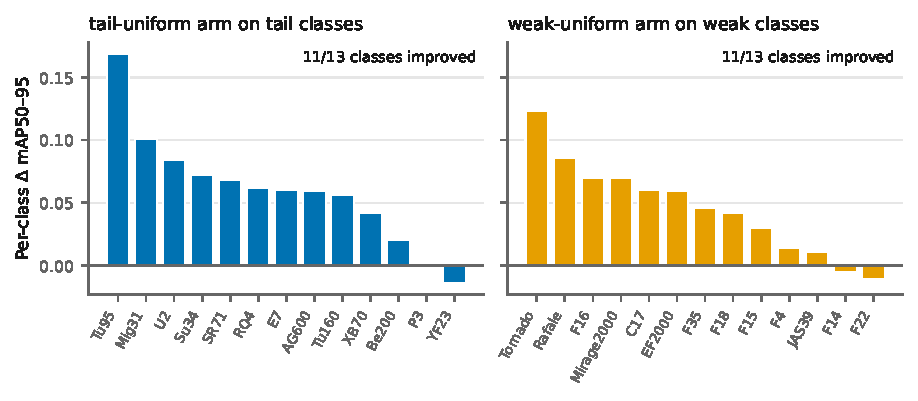
\includegraphics[width=\linewidth]{figures/fig6_perclass_delta.pdf}
\caption{Per-class gains are broad rather than concentrated. Sorted
per-class $\Delta$ \mapm{} (3-seed means) of the two uniform arms on
their targeted MAD classes; 11 of 13 classes improve in each set.}
\label{fig:perclass}
\end{figure}

\begin{figure}[t]
\centering

\includegraphics[width=\linewidth]{figures/fig3_dissociation.pdf}
\caption{The allocation signal shapes where gains occur. $\Delta$
\mapm{} versus the same-cell baseline for the four inpainting arms on
the tail scope (blue) and weak scope (orange); black-edged bars mark
each arm's targeted scope; error bars span $\pm 1$ standard deviation
over three seeds. Left: MAD (confirmatory; interaction Holm-adjusted
$p = 0.017$). Right: MAR20 (cross-dataset replication;
Section~\ref{sec:r1}).}
\label{fig:dissoc}
\end{figure}

\paragraph{The dissociation replicates in the satellite domain (MAR20)}
Figure~\ref{fig:dissoc} (right) shows the same analysis for MAR20 with
YOLOv8n. The interaction estimate was $+0.0523$ (95\% CI
$[0.021, 0.083]$; positive in all three seeds), close to the MAD
estimate ($+0.052$ vs.\ $+0.060$); the tail-targeted arm again gained
most on the tail scope (tail-priority: $+0.044$; descriptively, all six
tail classes improved) and the weak-targeted arms most on the weak
scope ($+0.030$ to $+0.034$). With only three seed blocks the
confirmatory test is low-powered --- and each MAR20 scope averages over
only six classes, which makes the per-seed macro scores noisier --- so
the interaction does not survive Holm correction (unadjusted
$p = 0.018$, Holm-adjusted $p = 0.091$). We therefore report MAR20 as a
cross-dataset replication of the direction with a similar point
estimate, without multiplicity-adjusted significance, rather than a
second confirmatory result.

\paragraph{Within-set weighting shows no benefit}
In contrast to the choice of class set, \emph{how} the fixed budget is
divided inside the chosen set showed no evidence of benefit in any
condition: the priority-versus-uniform contrasts were null in all four
pre-specified comparisons, with estimates centred near zero ($+0.002$
and $-0.012$ on MAD, $+0.014$ and $+0.004$ on MAR20; Holm-adjusted
$p = 0.808$, $0.345$, $0.336$, and $0.519$;
Table~\ref{tab:contrasts}). The CIs do
not exclude small effects in either direction, so we do not claim
strict equivalence; they do, however, exclude a priority advantage as
large as the set-choice effect. Given that the uniform and priority
arms shared the same class sets, generator, prompts, quality
verification, and budget, we conclude that at the budgets studied the
allocation \emph{signal} (which classes) --- not the allocation
\emph{shape} (how many per class) --- was the factor with detectable
effects.

\paragraph{Targeted gains come with smaller off-target gains}
Augmenting one set also produced consistent but smaller gains outside
it: on MAD the tail-uniform arm improved the weak scope by $+0.031$
(unadjusted class-level $p = 0.002$), and on MAR20 the cross-set gains
ranged from $+0.004$ to $+0.013$. We report this as an observation
without attributing a mechanism: because every annotated object in a
source image is retained, 21--44\% of accepted MAD synthetic images and
92--93\% of accepted MAR20 synthetic images contain objects of
non-target classes, so the present design cannot distinguish
background-mediated transfer from additional exposure to co-occurring,
non-target objects whose labels were retained
(Section~\ref{sec:discussion}).

\subsection{No measured arm shows a supported gain under the stronger pretrained detector}\label{sec:r2}

Replacing the compact detector with RT-DETR-L raised the
standard-augmentation baseline from 0.575 to 0.869 on MAD and from
0.572 to 0.697 on MAR20 --- and produced no statistically supported
gain among the measured arms (Figure~\ref{fig:condmap},
Table~\ref{tab:master}). On MAD, all all-scope mean deltas were
non-positive: tail-uniform $-0.004$, tail-priority $-0.001$, and RFS
$-0.016$; the pooled inpainting-versus-baseline contrast on the tail
scope was $-0.008$ (95\% CI $[-0.039, 0.022]$, Holm-adjusted
$p = 1.00$). On MAR20 the pattern repeated (tail-uniform $-0.007$,
tail-priority $-0.005$, RFS $+0.003$ on the all scope; pooled tail
contrast $+0.004$, 95\% CI $[-0.019, 0.026]$, Holm-adjusted $p = 0.66$). All three pre-specified contrasts of each
reduced cell are reported in Table~\ref{tab:contrasts}. We found no
evidence of a positive augmentation effect,
although the wide three-seed confidence intervals do not establish
equivalence to zero. Notably, the strong detector's \texttt{basic\_aug}
baseline already exceeded the best augmented YOLOv8n result by a wide
margin (0.869 vs.\ 0.661 on MAD).

Two observations follow. First, augmentation gains in this study were
confined to the lower-baseline compact detector: in the two
higher-baseline RT-DETR-L cells, no measured arm produced a supported
gain. This pattern is consistent with a headroom account, but headroom
is not a directly measured variable --- the MAR20 transformer baseline
(0.697) is far from any performance ceiling --- and the two detectors
differ simultaneously in architecture, capacity, and training recipe,
so we do not attribute the null to a single cause. In these
experiments, switching to RT-DETR-L coincided with a much larger
performance difference than any augmentation decision (a cross-cell
comparison; Section~\ref{sec:rules}). Second, the arm with the most
negative mean deltas under the strong detector was RFS on MAD
($-0.016$ all, $-0.010$ tail, $-0.016$ weak), although not uniformly
across seeds (one of three seeds was marginally positive on the all
scope); we report this as an observation without claiming a mechanism.
Because the RT-DETR-L cells implemented a reduced design (baseline,
RFS, and the two tail-set arms only), the weak-targeted arms were not
measured and no interaction test is available there; the null result
therefore covers the measured tail-targeted and resampling arms.

\begin{figure}[t]
\centering

\includegraphics[width=0.9\linewidth]{figures/fig4_condition_map.pdf}
\caption{Condition map across the four cells (descriptive, not a
formal test). $\Delta$ \mapm{} (all scope) against the same-cell
\texttt{basic\_aug} baseline; triangles denote repeat-factor sampling,
circles the tail-uniform arm --- the one inpainting arm trained in
every cell; color denotes the dataset. Mean deltas cluster near zero under the
high-baseline RT-DETR-L cells (right), and resampling and inpainting
exchange ranks between MAD and MAR20 (left).}
\label{fig:condmap}
\end{figure}

\subsection{Resampling effectiveness differs between the two dataset regimes}\label{sec:r3}

Repeat-factor sampling --- the generation-free exposure comparator
that produced larger mean deltas than every diffusion arm on MAD ($+0.086$ all, $+0.098$ tail,
$+0.117$ weak; unadjusted class-level $p \leq 2\times10^{-4}$) --- transferred
poorly to MAR20. With the same detector and protocol, RFS on MAR20
yielded $+0.003$ (all), $+0.016$ (tail), and $-0.011$ (weak;
unadjusted class-level $p = 0.031$) --- the only negative augmentation
effect to reach nominal significance in the class-level tests under
YOLOv8n. One possible interpretation is that re-exposing rare-class images
carries additional training signal under MAD's deep imbalance (max/min
instance ratio 10.5) and adds little under MAR20's shallower 20-class
distribution, while inpainting --- which injects genuinely new
background variation --- remains effective (Section~\ref{sec:r1});
because the datasets differ in more than imbalance, we treat this as
an interpretation rather than an established mechanism. On MAR20, inpainting was in fact the only
augmentation whose gains were consistently positive across arms and
scopes (Table~\ref{tab:master}). The practical
implication is developed in Section~\ref{sec:discussion}: RFS is a
simple first attempt rather than a universal winner, and in our two
datasets its failure coincided with the regime where generative
augmentation still helped.

\subsection{Robustness checks}\label{sec:robust}

\paragraph{Generation quality is unlikely to be the sole explanation}
The three originally generated MAD pools passed rule-based quality
verification at similar rates (79--82\%), and the fourth pool reached
its quota under the same criteria. Per-pool Fr\'{e}chet inception
distance \citep[FID;][]{heusel2017fid} and CLIP-based image--text
similarity \citep{radford2021clip}, computed for the three originally
generated pools, were comparable (method and per-pool values in
Appendix~\ref{app:audit}), and the \emph{worst}-FID pool
(weak-priority) nevertheless produced its targeted weak-scope gain
($+0.034$; Table~\ref{tab:master}); quality differences are therefore
unlikely to be the sole explanation for where gains landed. On
MAR20 the verification failure rates were 0.6--1.2\% per pool, and
all four pools reached the full 500-image budget.

\paragraph{Hallucinated objects do not drive the RFS gap on MAD}
A detector-based paired audit flagged a net increase in off-mask
detections --- candidate hallucinated aircraft --- in 10.2\% of
sampled MAD synthetic backgrounds (see Figure~\ref{fig:examples}, top
row).
Removing all detector-flagged images with an object-level gate and
retraining
the three original diffusion arms changed their all-scope performance by
at most $|\Delta| \leq 0.017$ (all nine gated-versus-ungated comparisons
non-significant in unadjusted class-level tests, $p = 0.11$--$0.97$);
because the gate also shrinks the three pools by different amounts (82,
85, and 165 images), this sensitivity analysis does not separate
label-noise removal from the accompanying budget reduction. The RFS
advantage persisted essentially unchanged ($\Delta = -0.055$ to $-0.067$ versus RFS,
unadjusted class-level $p < 10^{-4}$). A full-corpus gate scan removed 332 of the 3{,}000
images (11.1\%; 845 flagged extra detections), consistent with the
audit-sample estimate; per-pool statistics and the gated retraining
results are given in \ref{app:audit}. In the limited gated retraining (three arms, one matched seed),
removing the affected images therefore did not eliminate either the
dissociation pattern or the resampling gap.

\begin{figure}[t]
\centering

\includegraphics[width=0.8\linewidth]{figures/fig5_generation_examples.pdf}
\caption{Generation examples (source, protection mask, output; mask
black = protected). Rows: two MAD and two MAR20 cases spanning
formation, airshow, apron, and airbase scenes. The top row also
illustrates the hallucination failure mode quantified in
Section~\ref{sec:robust} --- diffusion has painted additional, unlabeled
aircraft into the regenerated sky --- which motivates the detector-based
audit and the object-gate robustness check.}
\label{fig:examples}
\end{figure}

\section{Discussion}\label{sec:discussion}

\subsection{Engineering guidance: a three-step decision rule}\label{sec:rules}

Read together, the four cells yield an actionable procedure for
practitioners who must decide whether --- and how --- to spend a
synthetic-data budget on a detection system.

\paragraph{Step 1: assess detector headroom before investing in
augmentation}
The largest single improvement observed in this study came not from any
data intervention but from replacing the detector: the pretrained
transformer's \texttt{basic\_aug} baseline exceeded the best augmented
result of the compact detector by 0.21 \mapm{} on MAD (0.869 vs.\
0.661), and once the stronger detector was in place, no measured
augmentation showed a supported gain and the RFS mean deltas on MAD
were negative (Section~\ref{sec:r2}). We stress that this is a cross-cell engineering
observation rather than a randomized comparison --- the two detectors
differ simultaneously in capacity and architecture family (both are
initialized from COCO-pretrained weights) --- but its practical reading
held in every condition we tested: when deployment constraints permit a
stronger pretrained detector, the model upgrade dominated every
augmentation decision we evaluated. Data-side interventions become
worth considering primarily where a compact detector is mandated, for
example by edge-compute budgets, and the model therefore retains
visible headroom.

\paragraph{Step 2: use generation-free resampling as a first attempt --- and as a practical probe}
Repeat-factor sampling requires no generation compute and, on the deeply
imbalanced MAD (imbalance ratio 10.5), outperformed every diffusion arm
on every scope (Section~\ref{sec:r3}). Its benefit did not transfer to
the shallowly imbalanced MAR20, where it was null overall and negative
on the weak scope. Because resampling can only re-expose existing
images, a natural reading is that it helps when under-exposure of rare
classes is the binding constraint and fails when the constraint lies
elsewhere; our two datasets are consistent with this reading but cannot
establish it, because they differ in more than imbalance
(Section~\ref{sec:design}).
Because materialized RFS changes the number of samples processed per
epoch, especially on MAD, this comparison is not compute- or
exposure-matched to the synthetic arms. In practice, RFS functions as a
simple exposure probe: run it first, keep it if
it helps, and treat a null result as a
practical prompt to consider a generative budget, not as a diagnosis
of the underlying cause.

\paragraph{Step 3: when generating, select the class set by
measured difficulty; uniform quotas are a reasonable default}
The interaction result (Section~\ref{sec:r1}) shows that the allocation
signal shapes where gains occur, whereas the within-set weighting
axis was null in all four pre-specified comparisons. This simplifies
deployment: in our experiments, the choice with detectable
consequences was which classes to target. Frequency is the conventional default for that choice, but it
is a poor one whenever frequency and difficulty decouple, as they do
here ($r = -0.373$). If the operational goal is to improve currently low-performing
classes, the per-class validation AP of the current baseline ---
available at no additional cost in any trained system --- is the direct
signal, and targeting the lowest-AP classes aligns the expected gains
with that goal; within the chosen set, a
uniform split showed no supported disadvantage and is the more
parsimonious default. The compute cost is moderate: generating and verifying one
thousand 512-pixel background variants took a few GPU-hours on a single
mid-range accelerator in our experiments, of the same order as one
detector training run at this scale.

\subsection{Why background inpainting behaves this way}\label{sec:mechanism}

Three observations jointly constrain the interpretation. First, the
compact detector's dominant error mode on MAD is missed detection:
baseline recall (0.52--0.59) trails precision (0.62--0.71), and the
largest off-diagonal mass in the confusion structure assigns true
objects to background (Figure~\ref{fig:confusion} in \ref{app:audit}). Second, gains concentrate on the targeted set yet
consistently spill over, attenuated, to non-targeted classes
(Section~\ref{sec:r1}). Third, no measured gain
is statistically supported under the higher-capacity pretrained
detector (Section~\ref{sec:r2}). These observations are consistent with one plausible account:
background inpainting may mitigate \emph{background overfitting}. Re-rendering the surroundings
of a geometrically protected object weakens context cues spuriously
correlated with class identity, potentially encouraging the detector to rely on object appearance
and thereby recover missed detections --- most strongly
for classes whose contexts were re-rendered (targeting), positively but
more weakly for classes that share the diversified background statistics
(spillover), and not at all for a detector with the capacity to retain
the broad variation of its pretraining, in which any spurious
object--context coupling is plausibly already weak (headroom). The account is also
consistent with a saturation reading of the null within-set contrasts:
once a class
receives enough background variation to break the spurious correlation,
additional variants of the same kind contribute little. Consistent with this reading, the tail-priority arm --- whose
smallest realized per-class quota was 16 images against the uniform
arm's 77 --- achieved statistically indistinguishable tail-scope
gains.
Finally, the MAR20 contrast between null resampling and effective
inpainting argues against re-exposure of the protected objects as the sole
driver of the gains --- the synthetic images repeat foregrounds nearly
unchanged (up to JPEG re-encoding), much as resampling does, yet only
the arm that also renews the backgrounds improved performance there
--- although the exposure counts of the two arms are not matched. The off-target component, in
particular, admits a second, exposure-based route --- co-occurring
non-target objects retained in the synthetic images
(Section~\ref{sec:r1}) --- which this design does not separate. We
advance this account as an interpretation consistent with all of our
observations, not as a demonstrated causal chain.

\subsection{Limitations and threats to validity}\label{sec:limitations}

Five limitations bound our claims. (1)~\emph{Replication power.} The
satellite-domain experiment reproduces the direction of the interaction
with a similar point estimate ($+0.052$ vs.\ $+0.060$), but with only
three seed blocks the confirmatory test is low-powered --- its
six-class scopes further add per-seed noise --- and the effect does not
survive Holm correction there; we accordingly claim replication of
direction and approximate magnitude, not a second confirmatory
result. (2)~\emph{Set
overlap.} On MAR20 the frequency-defined and difficulty-defined sets
share one of six classes, slightly diluting the dissociation relative to
the fully disjoint MAD design. (3)~\emph{Strong-detector cells: coverage
and attribution.} The transformer cells omit the weak-set arms, so the
headroom finding rests on near-zero deltas of the measured arms rather
than on an interaction test; moreover, the strong-detector comparison
co-varies capacity and architecture family (the pretraining corpus is
shared), so ``headroom'' names their joint effect rather than isolating
a single factor. The complete four-arm design on the strong detector,
together with capacity-matched comparisons within one architecture
family, would resolve both points. (4)~\emph{Training-period and split provenance.} In the MAD
compact-detector cell the reference runs predate the augmentation arms
(Section~\ref{sec:design}), so baseline-relative deltas there absorb
hardware-dependent batch resolution and Ultralytics-version drift
(8.4.87--8.4.115, recovered from checkpoint metadata), with the
remaining software environment unpreserved; the interaction contrast,
computed among contemporaneously trained arms, is unaffected. The MAD val/test halving is deterministic but not
stratified, and the web-collected images were not screened for
near-duplicates or
correlated scenes across splits. In addition, the three training seeds
of each arm share a single realization of its synthetic pool, so
generator-seed variability is not reflected in the seed-blocked
statistics.
(5)~\emph{External validity.} All evidence comes
from one application domain (aircraft), two datasets, one generator
family (Stable Diffusion inpainting, at one budget point per dataset),
and two detector capacity tiers. The condition map should therefore be
read as a demonstrated pattern with candidate moderators --- detector
headroom and imbalance depth --- not as a parametric law. Natural next
steps are budget scaling curves, a factorial combination of resampling
with targeted generation to test whether their gains compose, stronger
generators, and replication on broader long-tailed benchmarks. Targeted
retrieval from a large external real-image pool may also match or
outperform synthetic data in classification \citep{geng2024unmet}, but
that additional-data acquisition regime is not evaluated here and should
not be conflated with same-data RFS.

\section{Conclusion}\label{sec:conclusion}

We asked a question that the growing literature on generative
augmentation leaves implicit: when a fixed budget of synthetic images is
available, which classes should receive it? The complete four-arm crossed design, combining the allocation signal
with a within-set quota rule, ran on both public military-aircraft
benchmarks with the compact detector under a cell-specific fixed
budget, generator, and verification protocol; a reduced arm set then
probed transfer to a stronger pretrained detector. The answer is
consistent: class-set selection was the allocation decision with
detectable consequences --- gains were larger on, and shifted toward,
the targeted set, confirmed by a pre-specified interaction on the
natural-view benchmark and replicated in direction and approximate
magnitude on the satellite-view benchmark --- while priority weighting
showed no supported advantage over a uniform split at the tested
budgets. The choice of signal is not innocuous: frequency and measured
difficulty selected disjoint classes on MAD and largely distinct
classes on MAR20, and practitioners whose goal is to improve currently
low-performing classes should target the measured-weakest classes
rather than the rarest. Both findings are conditional: under the large
pretrained transformer none of the measured arms showed a supported
gain, and the generation-free resampling comparator that outperformed
generation on the deeply imbalanced benchmark was null overall on the
less imbalanced one, with a negative mean delta on its weak scope; we
do not attribute this contrast to imbalance depth alone. The resulting
decision rule --- assess baseline headroom, probe with resampling, then
generate for measured weakness with a uniform split --- provides a
practical, testable workflow, and the evaluation protocol behind it
(budget control, pre-specified contrasts, seed-blocked tests) is
reusable in controlled augmentation studies, particularly for
long-tailed detection. Extending the complete four-arm
design to strong detectors, tracing budget scaling curves, and testing
whether resampling and targeted generation compose are the natural next
steps.

%% ------------------------------------------------------------------
%% Declarations (EAAI). NOTE for double-anonymized submission: move the
%% author block, CRediT, and funding to a separate title page and keep
%% the manuscript body anonymized.
\section*{Declaration of competing interest}
The author declares no known competing financial interests or personal
relationships that could have appeared to influence the work reported
in this paper.

\section*{Funding}
%% TODO(user): confirm before submission.
This research did not receive any specific grant from funding agencies
in the public, commercial, or not-for-profit sectors.

\section*{CRediT authorship contribution statement}
\textbf{Daehyun Yoo}: Conceptualization, Methodology, Software,
Investigation, Formal analysis, Data curation, Writing -- original
draft, Writing -- review \& editing, Visualization.

\section*{Data availability}
Both source datasets are publicly available (MAD via Kaggle; MAR20 via
its official release). Configuration files, allocation plans,
generation logs, verification reports, contrast freezes, per-class
metrics, and code will be deposited in a public repository upon
acceptance. Redistribution of the generated image pools is contingent
on the source datasets' licence terms.
%% TODO(user): repository link + licence confirmation before submission.

\section*{Declaration of generative AI and AI-assisted technologies}
During the preparation of this work the author used AI coding
assistants (Anthropic Claude Code; OpenAI Codex) to draft and revise
manuscript text, to cross-check consistency between the manuscript and
the archived experimental artifacts, and to write figure and analysis
scripts. After using these tools, the author reviewed and edited the
content as needed and takes full responsibility for the content of the
published article.
%% TODO(user): confirm tool list wording.

\appendix
\section{Generation details}\label{app:gen}
\paragraph{Generator and revision}
All pools were generated with the \texttt{runwayml/stable-diffusion-inpainting} checkpoint. The confirmatory-phase generation runs resolved this model to Hugging Face snapshot \texttt{8a4288a76071f7280aedbdb3253bdb9e9d5d84bb} (recovered from the archived run logs), and the configuration files now pin this revision for regeneration. The three exploratory-phase pools used the same model identifier, but their runtime did not log the resolved revision, and the Diffusers/PyTorch versions of the generation environment were not preserved.
\paragraph{Scene and negative prompts}
The five scene prompts per dataset (rotated per generated image) and the dataset-specific negative prompts are reproduced verbatim below.
\begin{itemize}\small
\item[] \texttt{realistic sky background, natural lighting, aviation photography, high resolution, realistic clouds}
\item[] \texttt{realistic runway background, military airbase, natural lighting, aviation photography}
\item[] \texttt{cloudy sky background, realistic atmosphere, aviation photography}
\item[] \texttt{clear blue sky, sunlight, realistic aircraft photography}
\item[] \texttt{desert airfield background, haze, realistic lighting}
\item[] negative: \texttt{deformed aircraft, changed aircraft shape, extra aircraft, duplicate aircraft, new aircraft, distorted object, text, watermark, low quality, blurry}
\end{itemize}
\noindent\emph{(MAD)}\medskip
\begin{itemize}\small
\item[] \texttt{aerial satellite view of airport apron, concrete tarmac with faded lane markings, top-down view, high resolution satellite imagery}
\item[] \texttt{top-down aerial view of military airbase runway and taxiway, asphalt surface, satellite photography}
\item[] \texttt{overhead satellite view of dry grass and soil beside airport taxiway, realistic aerial imagery}
\item[] \texttt{top-down view of empty concrete aircraft parking stands, tire marks and oil stains, satellite imagery}
\item[] \texttt{aerial satellite view of desert airfield ground, sand and weathered pavement, overhead imagery}
\item[] negative: \texttt{aircraft, airplane, jet, extra aircraft, duplicate aircraft, deformed aircraft, vehicle, sky, clouds, horizon, oblique perspective, side view, text, watermark, low quality, blurry}
\end{itemize}
\noindent\emph{(MAR20)}
\paragraph{Class memberships}
\begin{table}[h]\centering\small
\caption{Tail and weak class memberships (weak sets for the compact detector).}
\begin{tabular}{lp{0.75\linewidth}}\toprule
MAD tail & AG600, Be200, E7, Mig31, P3, RQ4, SR71, Su34, Tu160, Tu95, U2, XB70, YF23 \\
MAD weak & C17, EF2000, F14, F15, F16, F18, F22, F35, F4, JAS39, Mirage2000, Rafale, Tornado \\
\midrule
MAR20 tail & A11, A15, A18, A4, A6, A7 \\
MAR20 weak & A1, A12, A15, A16, A19, A5 \\
\bottomrule\end{tabular}\end{table}
\paragraph{Realized allocation quotas}
\begin{table}[h]\centering\small\caption{Per-class quotas, MAD (left column pair: tail-set arms; right pair: weak-set arms).}
\begin{tabular}{lrr@{\qquad}lrr}\toprule
Class & unif. & prio. & Class & unif. & prio. \\ \midrule
Mig31 & 77 & 67 & C17 & 77 & 69 \\
RQ4 & 77 & 81 & EF2000 & 77 & 100 \\
Su34 & 77 & 76 & F14 & 77 & 65 \\
Be200 & 77 & 16 & F15 & 77 & 71 \\
U2 & 77 & 53 & F16 & 77 & 85 \\
SR71 & 77 & 36 & F18 & 77 & 67 \\
Tu95 & 77 & 61 & F22 & 76 & 64 \\
Tu160 & 77 & 65 & F35 & 77 & 69 \\
AG600 & 77 & 47 & F4 & 77 & 91 \\
XB70 & 77 & 124 & JAS39 & 77 & 98 \\
P3 & 77 & 127 & Mirage2000 & 77 & 69 \\
YF23 & 77 & 121 & Rafale & 77 & 78 \\
E7 & 76 & 126 & Tornado & 77 & 74 \\
\bottomrule\end{tabular}\end{table}
\begin{table}[h]\centering\small\caption{Per-class quotas, MAR20 (left column pair: tail-set arms; right pair: weak-set arms).}
\begin{tabular}{lrr@{\qquad}lrr}\toprule
Class & unif. & prio. & Class & unif. & prio. \\ \midrule
A15 & 84 & 100 & A1 & 84 & 98 \\
A7 & 84 & 56 & A5 & 83 & 78 \\
A4 & 83 & 44 & A12 & 83 & 81 \\
A11 & 83 & 100 & A15 & 84 & 89 \\
A18 & 83 & 100 & A16 & 83 & 75 \\
A6 & 83 & 100 & A19 & 83 & 79 \\
\bottomrule\end{tabular}\end{table}
\paragraph{Compute}
Total training compute on a single NVIDIA L4 (measured wall-clock per run, summed): MAD/YOLOv8n: 33.0\,GPU-h; MAD/RT-DETR-L: 34.4\,GPU-h; MAR20/YOLOv8n: 2.8\,GPU-h; MAR20/RT-DETR-L: 11.2\,GPU-h. Generating and verifying the four MAR20 pools (2{,}000 images) took 2.1\,GPU-h; a 1{,}000-image MAD pool takes approximately 3\,GPU-h on the same hardware.

\begin{figure}[h]\centering
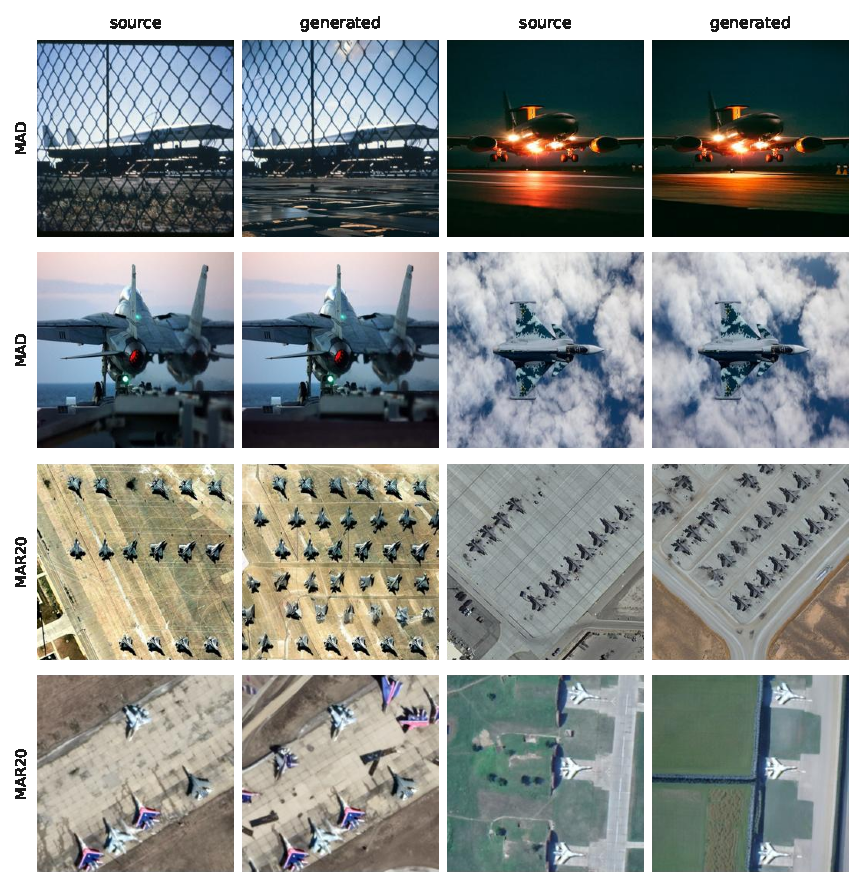
\includegraphics[width=0.92\linewidth]{figures/figa1_gallery.pdf}
\caption{Additional source/generated pairs (backgrounds regenerated;
all annotated objects protected). Top three rows: MAD; bottom row and
right half of row three: MAR20.}
\label{fig:gallery}
\end{figure}

\section{Per-class results}\label{app:perclass}
\begin{table}[h]\centering\small\caption{MAD tail classes: baseline test \mapm{} and per-arm $\Delta$ (3-seed means).}\label{tab:pc-mad-tail}
\begin{tabular}{lrrrrrrr}\toprule
Class & $n$ & base & tail-unif. & tail-prio. & weak-unif. & weak-prio. & RFS \\ \midrule
YF23 & 97 & 0.801 & -0.014 & +0.001 & -0.022 & -0.004 & +0.040 \\
AG600 & 153 & 0.763 & +0.059 & +0.032 & +0.041 & +0.018 & +0.034 \\
Be200 & 209 & 0.757 & +0.020 & +0.012 & +0.023 & -0.003 & +0.078 \\
P3 & 118 & 0.712 & -0.000 & +0.051 & +0.000 & +0.004 & +0.063 \\
XB70 & 119 & 0.656 & +0.041 & +0.077 & +0.055 & +0.014 & +0.103 \\
Mig31 & 225 & 0.636 & +0.101 & +0.101 & -0.006 & -0.010 & +0.132 \\
SR71 & 206 & 0.627 & +0.068 & +0.054 & +0.040 & +0.046 & +0.131 \\
Tu160 & 192 & 0.598 & +0.056 & +0.125 & +0.055 & +0.060 & +0.163 \\
E7 & 86 & 0.592 & +0.060 & +0.065 & +0.001 & +0.036 & +0.045 \\
Su34 & 210 & 0.565 & +0.072 & +0.058 & +0.030 & +0.075 & +0.045 \\
Tu95 & 197 & 0.505 & +0.169 & +0.132 & -0.042 & +0.110 & +0.144 \\
U2 & 208 & 0.439 & +0.084 & +0.088 & -0.015 & +0.009 & +0.106 \\
RQ4 & 212 & 0.404 & +0.062 & +0.010 & +0.027 & +0.030 & +0.194 \\
\bottomrule\end{tabular}\end{table}
\begin{table}[h]\centering\small\caption{MAD weak classes: baseline test \mapm{} and per-arm $\Delta$ (3-seed means).}\label{tab:pc-mad-weak}
\begin{tabular}{lrrrrrrr}\toprule
Class & $n$ & base & tail-unif. & tail-prio. & weak-unif. & weak-prio. & RFS \\ \midrule
Tornado & 273 & 0.561 & +0.047 & +0.048 & +0.123 & +0.096 & +0.106 \\
F4 & 411 & 0.555 & -0.026 & -0.036 & +0.014 & -0.015 & +0.052 \\
F35 & 746 & 0.518 & +0.029 & +0.035 & +0.046 & +0.076 & +0.066 \\
Mirage2000 & 297 & 0.513 & +0.041 & +0.039 & +0.069 & +0.056 & +0.183 \\
F15 & 851 & 0.481 & +0.014 & +0.032 & +0.030 & +0.023 & +0.106 \\
EF2000 & 388 & 0.475 & +0.053 & -0.015 & +0.059 & +0.048 & +0.158 \\
F16 & 902 & 0.468 & +0.048 & +0.028 & +0.070 & +0.046 & +0.095 \\
C17 & 348 & 0.465 & +0.013 & +0.026 & +0.060 & +0.068 & +0.148 \\
F22 & 450 & 0.450 & +0.032 & -0.004 & -0.011 & -0.018 & +0.004 \\
JAS39 & 350 & 0.428 & +0.018 & +0.013 & +0.010 & +0.024 & +0.193 \\
F18 & 885 & 0.416 & +0.022 & +0.013 & +0.042 & +0.024 & +0.091 \\
F14 & 358 & 0.331 & +0.030 & -0.129 & -0.006 & -0.040 & +0.177 \\
Rafale & 369 & 0.269 & +0.078 & +0.039 & +0.086 & +0.048 & +0.137 \\
\bottomrule\end{tabular}\end{table}
\begin{table}[h]\centering\small\caption{MAR20 (all 20 classes): baseline test \mapm{} and per-arm $\Delta$ (3-seed means).}\label{tab:pc-mar20}
\begin{tabular}{lrrrrrrr}\toprule
Class & $n$ & base & tail-unif. & tail-prio. & weak-unif. & weak-prio. & RFS \\ \midrule
A7 & 150 & 0.743 & +0.022 & +0.015 & +0.023 & -0.007 & -0.008 \\
A17 & 360 & 0.738 & -0.008 & +0.005 & -0.017 & -0.017 & +0.005 \\
A10 & 305 & 0.686 & -0.005 & -0.003 & -0.015 & -0.013 & -0.016 \\
A2 & 590 & 0.678 & +0.002 & +0.000 & -0.022 & -0.018 & -0.005 \\
A6 & 84 & 0.673 & +0.016 & +0.028 & +0.011 & -0.002 & +0.029 \\
A8 & 289 & 0.658 & -0.015 & +0.006 & -0.035 & -0.041 & +0.008 \\
A9 & 418 & 0.652 & +0.000 & -0.002 & -0.029 & -0.031 & -0.019 \\
A14 & 536 & 0.647 & +0.003 & +0.012 & -0.011 & -0.007 & +0.004 \\
A4 & 149 & 0.627 & +0.058 & +0.066 & +0.034 & +0.038 & +0.057 \\
A3 & 252 & 0.617 & +0.038 & +0.030 & +0.004 & -0.003 & +0.029 \\
A1 & 441 & 0.605 & -0.046 & -0.062 & -0.014 & -0.017 & -0.017 \\
A12 & 198 & 0.603 & -0.021 & -0.027 & +0.005 & +0.009 & -0.001 \\
A20 & 350 & 0.558 & -0.008 & -0.018 & +0.014 & +0.015 & +0.009 \\
A16 & 648 & 0.524 & +0.047 & +0.057 & +0.074 & +0.077 & -0.010 \\
A11 & 127 & 0.517 & -0.006 & +0.030 & -0.017 & -0.032 & -0.015 \\
A19 & 394 & 0.512 & +0.008 & -0.016 & +0.022 & +0.016 & -0.003 \\
A13 & 463 & 0.426 & +0.005 & -0.016 & +0.008 & +0.016 & +0.006 \\
A18 & 117 & 0.419 & +0.011 & +0.049 & -0.045 & -0.048 & +0.044 \\
A5 & 366 & 0.343 & +0.014 & +0.021 & +0.049 & +0.045 & -0.022 \\
A15 & 165 & 0.214 & +0.079 & +0.072 & +0.044 & +0.073 & -0.011 \\
\bottomrule\end{tabular}\end{table}
\section{Generation quality, hallucination audit, and object-level gate}\label{app:audit}
\paragraph{Quality metrics}
FID (torchmetrics FrechetInceptionDistance, Inception-V3 features) is computed per pool against the real training images containing that pool's target classes, so the reference sets differ across pools and cross-pool FID is indicative rather than strictly comparable; CLIPScore (\texttt{openai/clip-vit-base-patch16}) measures image--prompt similarity and LPIPS (AlexNet backbone) measures source--output distance, both on 200 sampled images per pool. The metrics were computed in the exploratory phase and therefore cover the three originally generated pools; the weak-uniform pool, generated later in the confirmatory phase, passed the same rule-based verification but was not scored.
\begin{table}[h]\centering\small\caption{Per-pool quality metrics (three exploratory-phase MAD pools).}\label{tab:quality}
\begin{tabular}{lrrrr}\toprule
Pool & FID & FID ref.\ ($n$ real) & CLIPScore & LPIPS \\ \midrule
tail-uniform & 89.7 & 1,797 & 19.6 $\pm$ 3.3 & 0.262 \\
tail-priority & 87.7 & 1,797 & 19.1 $\pm$ 3.8 & 0.244 \\
weak-priority & 100.4 & 3,744 & 20.2 $\pm$ 3.4 & 0.272 \\
\bottomrule\end{tabular}\end{table}
A detector-based scan of all 3{,}000 MAD synthetic images (the three originally generated pools) flagged images containing hallucinated, unlabeled aircraft. Table~\ref{tab:gate} reports per-pool removal statistics; a detector-based paired audit of a 450-image sample (150 per pool) flagged a net increase in off-mask detections in 10.2\% of images, consistent with the 11.1\% full-scan removal rate.
\begin{table}[h]\centering\small\caption{Object-level gate: full-corpus scan of the MAD pools.}\label{tab:gate}
\begin{tabular}{lrrrr}\toprule
Pool & images & removed & removed (\%) & flagged objects removed \\ \midrule
tail-priority & 1000 & 82 & 8.2 & 159 \\
tail-uniform & 1000 & 85 & 8.5 & 170 \\
weak-priority & 1000 & 165 & 16.5 & 516 \\
\midrule total & 3000 & 332 & 11.1 & 845 \\
\bottomrule\end{tabular}\end{table}
Retraining the three arms on gated pools (seed matched to the ungated runs) changed macro \mapm{} only marginally:
\begin{table}[h]\centering\small\caption{Gated $-$ ungated macro \mapm{} (single matched seed).}\label{tab:gated}
\begin{tabular}{lrrr}\toprule Arm & all & tail & weak \\ \midrule
tail-uniform & +0.005 & +0.009 & -0.009 \\
tail-priority & -0.017 & -0.012 & -0.021 \\
weak-priority & -0.001 & -0.002 & -0.008 \\
\bottomrule\end{tabular}\end{table}

\begin{figure}[h]\centering
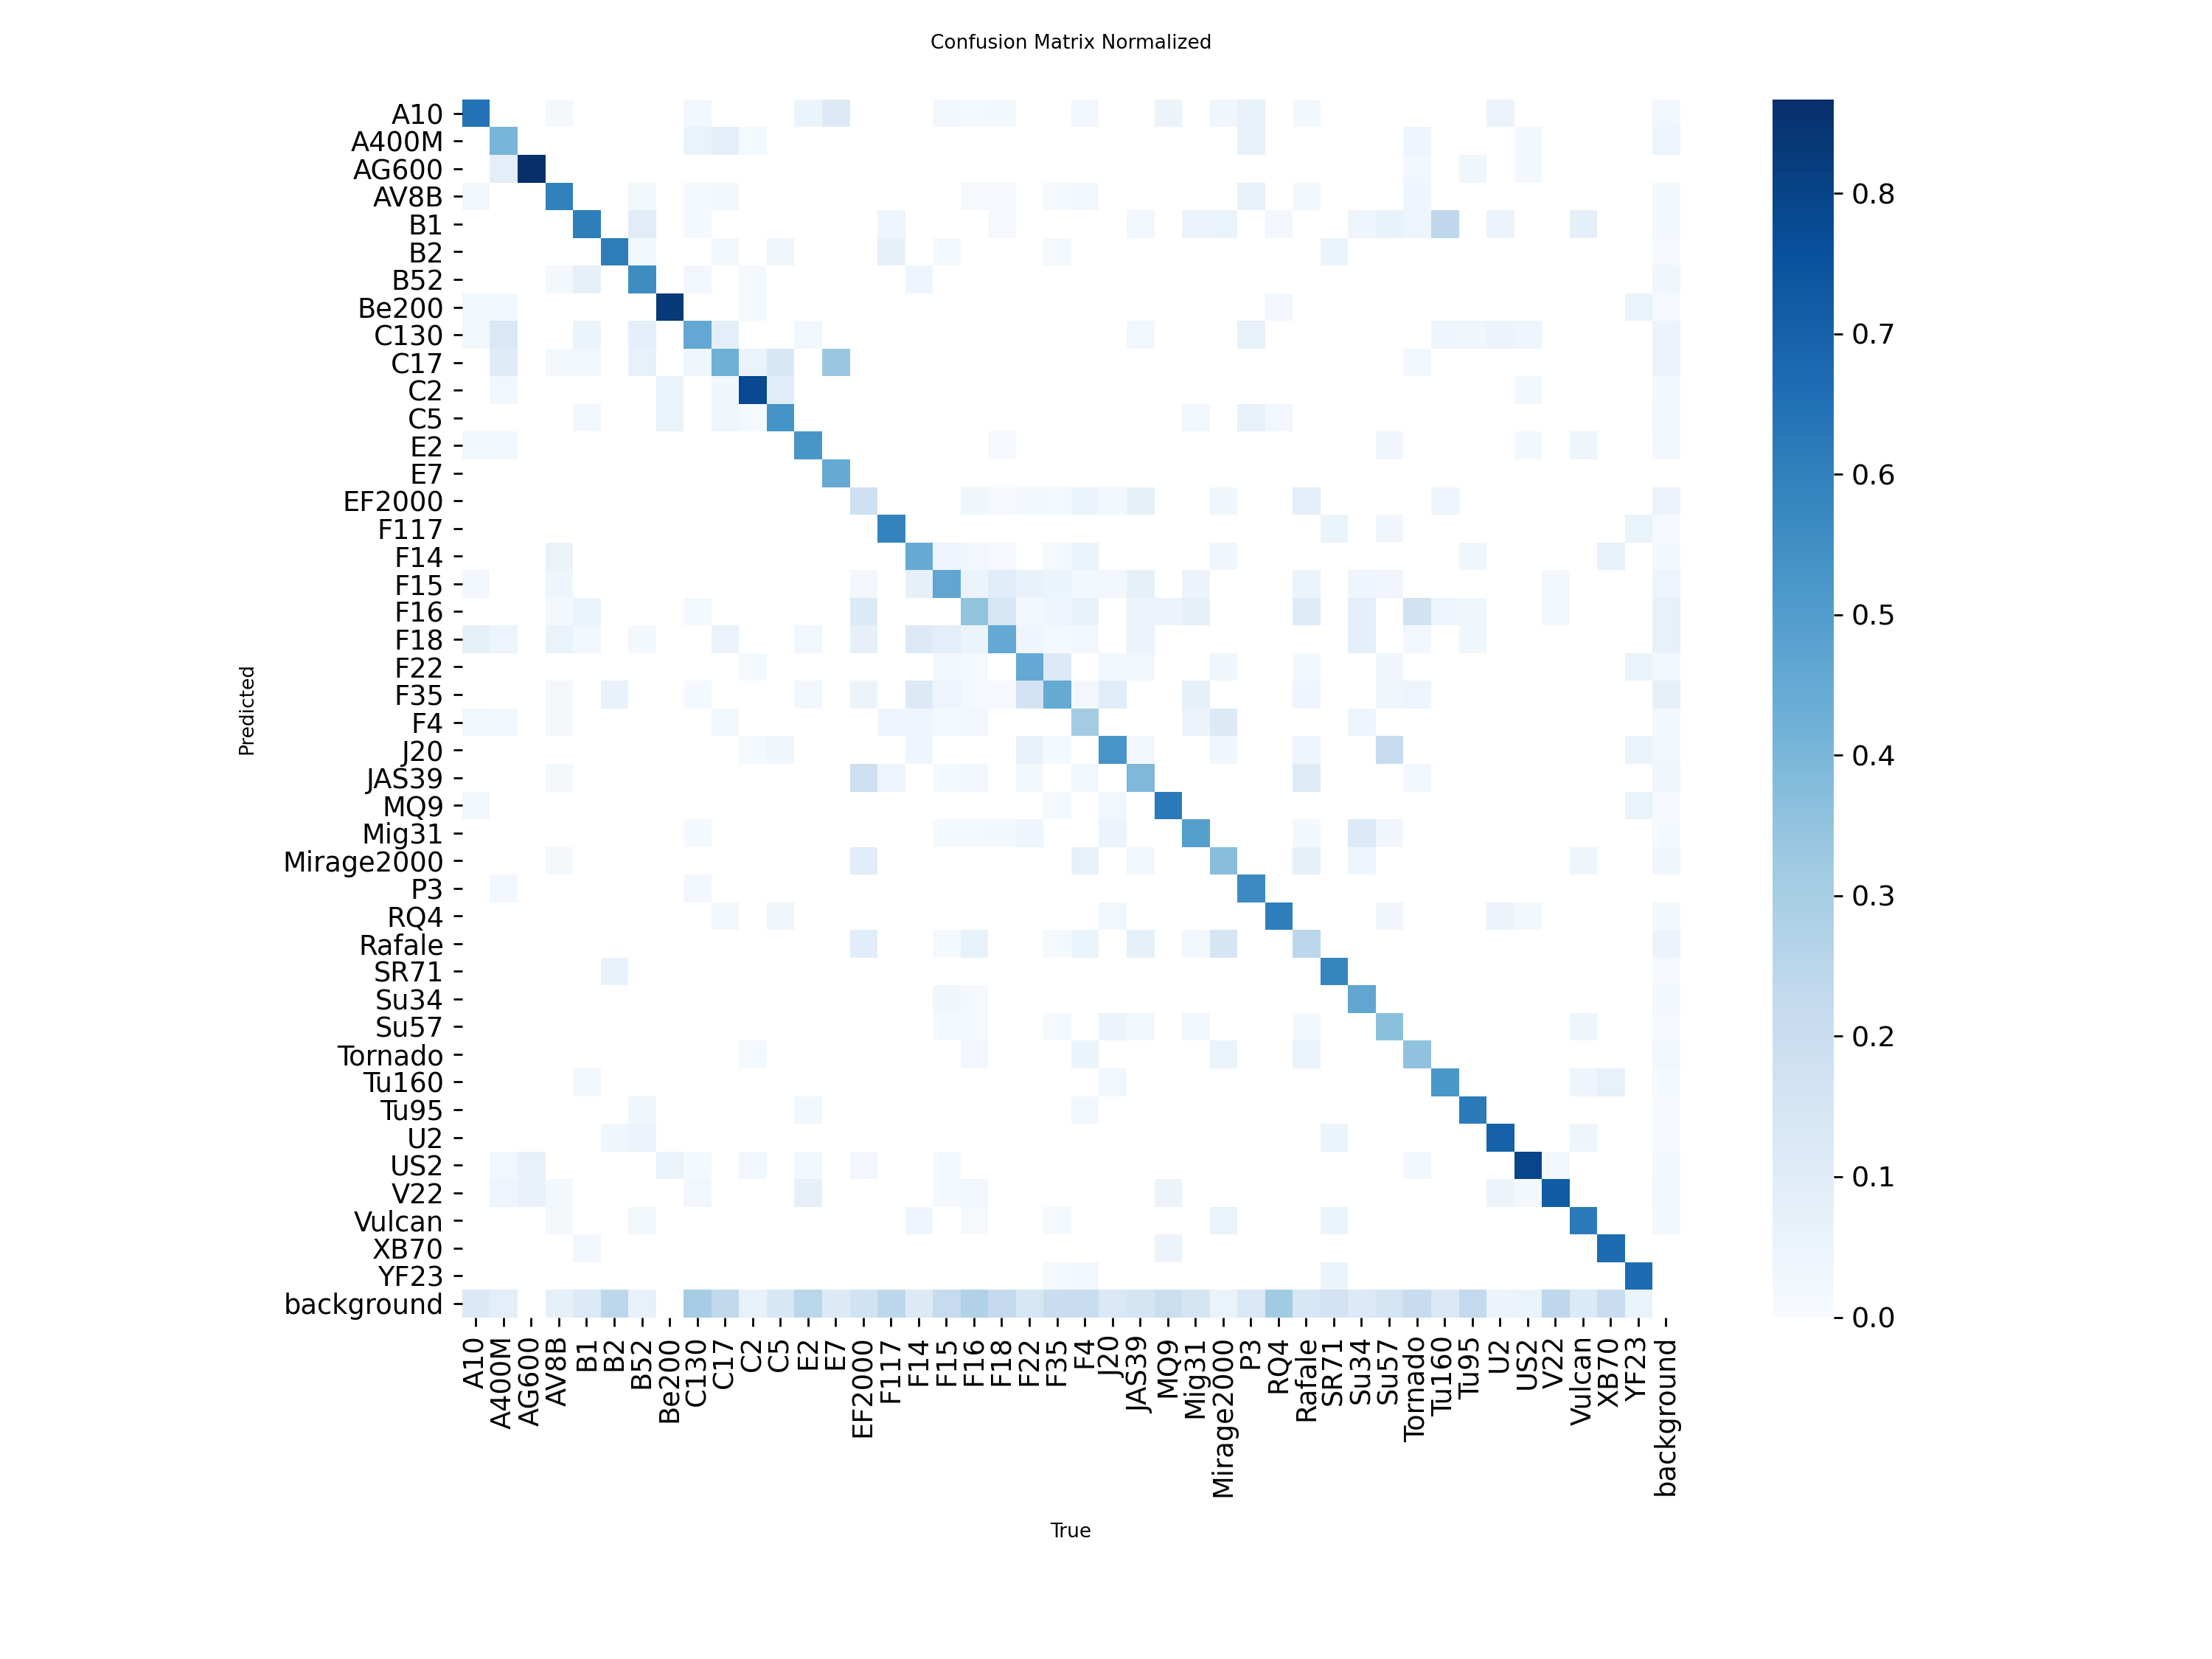
\includegraphics[width=0.9\linewidth]{figures/figa2_confusion.png}
\caption{Normalized confusion matrix of the MAD \texttt{basic\_aug}
baseline (one seed). The dominant off-diagonal mass lies in the
background row (missed detections), the error mode hypothesized to be
affected by background diversification (Section~\ref{sec:mechanism}).}
\label{fig:confusion}
\end{figure}



\bibliographystyle{elsarticle-harv}
\bibliography{refs}

\end{document}
